\documentclass[accentcolor=tud9d,colorbacktitle,inverttitle,landscape,german,presentation,t]{tudbeamer}
\usepackage{ngerman}
\usepackage{graphicx}

\begin{document}

	% Titel
	\title{Instant Message Whispering \\via Covert Channels}
	\subtitle{Martin Oehler}
	
 	% Fußzeile
	\author{Martin Oehler}
	\date{\today}

\begin{titleframe}
	
\includegraphics[scale=.5]{Bilder/InstantMessenger.jpg}
\end{titleframe}

\begin{frame}
	\frametitle{Einf"uhrung}

	Verstecktes Instant Messaging
	\begin{itemize}
		\item Senden von Nachrichten durch Firewalls
		\item Vermeiden von Entdeckung, Abh"oren und Abfangen
	\end{itemize}
	\textbf{} \newline
	
	\begin{description}
		\item[Kryptographie:] Verschl"usselt die Daten, Kanal bleibt sichtbar
		\item[Covert Channels:] Versteckt den Kanal
	\end{description}
	
	\begin{center}
	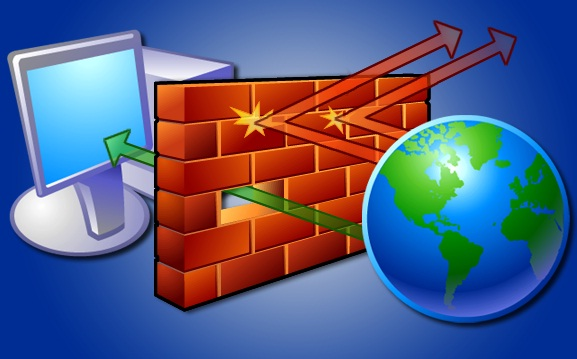
\includegraphics[scale=.3]{Bilder/Firewall.jpg}
	\end{center}
	
\end{frame}

\begin{frame}

	\frametitle{Projektbeschreibung}
	Programmieren einer Bibliothek f"ur Covert Channels
	\begin{itemize}
		\item "Offnet und verwendet Covert Channels
		\item Implementierung eines Frameworks
		\item Konkrete Covert Channels als Plugin
		\item Ver"offentlichung als Open Source
	\end{itemize}
	\begin{center}
	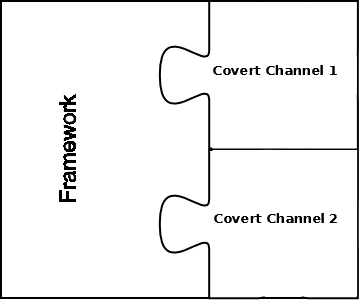
\includegraphics[scale=0.25]{Bilder/framework-puzzle.png}
	\end{center}

\end{frame}

\begin{frame}

	\frametitle{QS-Ziele}
	\begin{itemize}
		\item Modularit"at \\
		\only<2>{Modulares Design des Framework mit festen Modulschnittstellen}
		\item Zuverl"assigkeit \\
		\only<3>{Testdriven Developement als Entwicklungsmodell}
		\item Testbarkeit	\\
		\only<4>{Separation of concerns }
	\end{itemize}

\end{frame}

\begin{frame}
	\frametitle{Zeitsumme}
	\textbf{Gesamtsumme: 8 Stunden}
	\begin{center}
		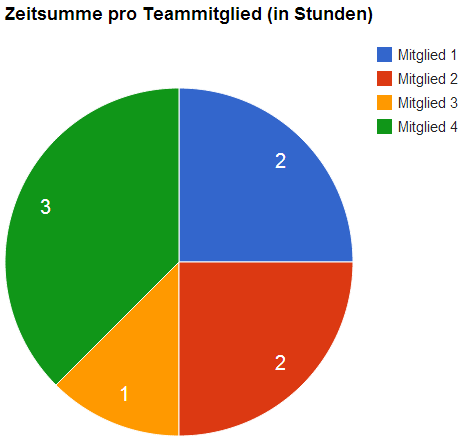
\includegraphics[scale=0.5]{Bilder/zeitsummen.png} \newline
	\end{center}

\end{frame}

\begin{frame}
\frametitle{Zeitmanagement}
	\begin{center}
		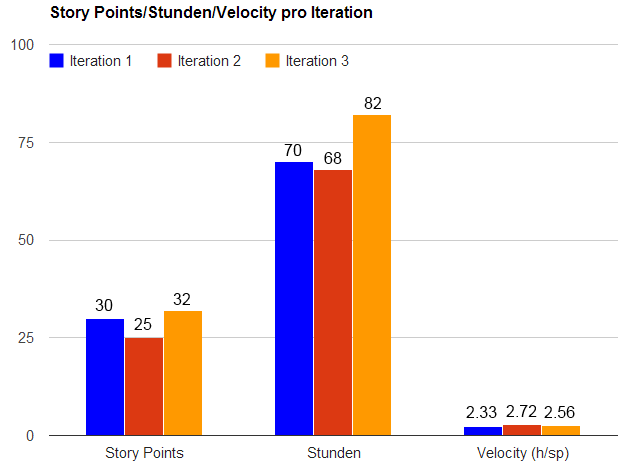
\includegraphics[scale=.5]{Bilder/iteration.png}
	\end{center}

\end{frame}

\begin{frame}
\frametitle{Ende}

Vielen Dank f"ur Ihre Aufmerksamkeit.
\end{frame}

\end{document}